\section{Design Philosophy and System Architecture}
\label{sec:system_overview}

The design brings several everyday functions into a display that users can configure and maintain after installation. A teacher may use it for an examination countdown, while office staff may use the same device for a notice or ordinary timekeeping. Changing its role should require changing its configuration through a browser. This guided the choice to combine display functions, network setup, persistent configuration, and firmware maintenance within one microcontroller-based system.

\begin{figure*}[t]
\centering
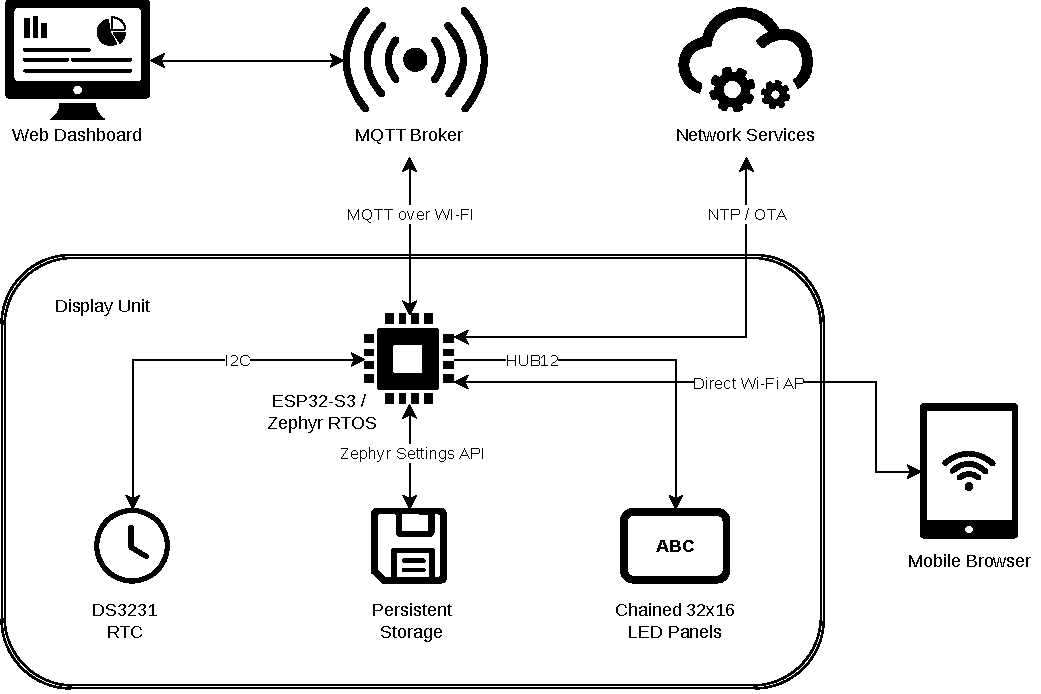
\includegraphics[width=\textwidth]{figs/architecture.pdf}
\caption{System architecture combining remote management with local display execution. The mobile browser provides a direct connection for Wi-Fi provisioning, while network services supply time synchronization and firmware images.}
\label{fig:architecture}
\end{figure*}

Figure~\ref{fig:architecture} shows how these responsibilities are distributed. The web dashboard provides the management interface, and MQTT carries commands and device status. The ESP32-S3 interprets these commands and generates the displayed content locally. Clockfaces, scrolling notices, and timers share a display manager and framebuffer, with the chained panels presented through Zephyr's display interface. The same display also presents firmware-update progress. This arrangement supports the required text and timing functions without a Linux-capable controller or browser-based rendering on each unit.

Local execution includes deciding how an activity progresses over time. A scheduled timer is represented by its start and end timestamps, which are retained in persistent storage. During startup, the firmware compares these timestamps with the RTC: a future activity remains scheduled, an active activity resumes according to the current time, and an expired activity is cleared. For example, a countdown scheduled to finish at 11:00 should still finish at 11:00 after a restart at 10:20. Preserving the schedule therefore matters more than preserving the last number drawn on the screen.

Zephyr provides a common software foundation through its device interfaces, networking facilities, and settings subsystem. The chained panels are exposed through its display interface, keeping the application independent of the panel-driving details. We contributed the HUB12 driver to upstream Zephyr, allowing the panel interface to be reused independently of the clock application.

Installation and maintenance shaped the design alongside its display functions. Users need to connect a mounted unit to the local network, change its role, and install software updates without opening the enclosure. We therefore included browser-based provisioning and remote firmware updates as part of the device's normal operation.